% Header
%\documentclass[12pt,a4paper]{report}
\usepackage[utf8]{inputenc}
\usepackage[T1]{fontenc}
\usepackage{geometry}
\usepackage{graphicx}
\usepackage[danish]{isodate}
\usepackage[danish]{babel}
\usepackage{url}
\usepackage{color}
\usepackage{ulem}
\usepackage{titlesec}
\usepackage{hyperref}
\usepackage{float}

% Fonts
\usepackage{helvet} % <-- Helvetica (sans)
\usepackage[sc]{mathpazo} % <-- Palatino (serif)
\linespread{1.05}   % Extra linespread for Palatino

% Extra settings
% \setlength\parindent{0pt} % For at fjerne automatiske indrykninger
% \let\clearpage\relax % For at fjerne alle clearpage sideskift

% Commands
\newcommand{\code}[1]{\texttt{#1}}

% Meta (til titelblad)
% HUSK; at rette Jonas i titelbladet.
\newcommand{\rtitle}{Erstattes med rapportens titel} %<----
\newcommand{\rtheme}{Elektroniske Lommepenge}
\newcommand{\rperiod}{P2, 2013}
\newcommand{\rdeadline}{\today} %<----Erstattes med rapportens deadline
\newcommand{\rprints}{1} %<---- Erstattes med oplægsantal
\newcommand{\rappendices}{0} %<---- Erstattes med bilagsantal og art
\newcommand{\rlastpage}{} %<---- Erstattes med sideantal

%%Jonas
\usepackage{lastpage}

\documentclass[12pt,a4paper]{report}
\usepackage[utf8]{inputenc}
\usepackage[T1]{fontenc}
\usepackage{geometry}
\usepackage{graphicx}
\usepackage[danish]{isodate}
\usepackage[danish]{babel}
\usepackage{url}
\usepackage{color}
\usepackage{ulem}
\usepackage{titlesec}
\usepackage{hyperref}

% Fonts
\usepackage[scaled]{helvet} % <-- Helvetica (sans)
\usepackage[sc]{mathpazo} % <-- Palatino (serif)
\linespread{1.05}   % Extra linespread for Palatino

% Extra settings
% \setlength\parindent{0pt} % For at fjerne automatiske indrykninger
% \let\clearpage\relax % For at fjerne alle clearpage sideskift

% Meta (til titelblad)
% HUSK; at rette Jonas i titelbladet.
\newcommand{\rtitle}{Erstattes med rapportens titel} %<----
\newcommand{\rtheme}{Elektroniske Lommepenge}
\newcommand{\rperiod}{P2, 2013}
\newcommand{\rdeadline}{\today} %<----Erstattes med rapportens deadline
\newcommand{\rprints}{1} %<---- Erstattes med oplægsantal
\newcommand{\rappendices}{0} %<---- Erstattes med bilagsantal og art
\newcommand{\rlastpage}{} %<---- Erstattes med sideantal

%%Jonas
\usepackage{lastpage}





% Document root
\begin{document}

% AAU Titelblad
%\begin{titlepage}
  \newgeometry{top=1in,bottom=1in,right=1in,left=1in}
  % AAU Logo
  \begin{minipage}{0.40\textwidth}
  
\includegraphics[width=\textwidth]{Billeder/aau-logo-new.pdf}
  \end{minipage}
  \hfill
  \begin{minipage}{0.40\textwidth}
    {\sf\small \textbf{Det Teknisk-Naturvidenskabelige\\ Basis{\aa}r }}\\
    {\sf\small  \textbf{Datalogi og Software}} \\
    {\sf\small Strandvejen 12-14} \\
    {\sf\small Telefon 96 35 97 31} \\
    {\sf\small Fax 98 13 63 93} \\
    {\sf\small http://tnb.aau.dk}
  \end{minipage}
  
  \begin{minipage}{0.4\textwidth}
    \begin{description}
    \vspace{1cm}
    
    \item {\bf Titel:}\\ \rtitle
    
    \item {\bf Tema:}\\ \rtheme 
    
    \item {\bf Projektperiode:}\\ \rperiod
    
    \item {\bf Projektgruppe:}\\ A325
    
    \item {\bf Deltagere:}\\
    Bossen, Jannek Alexander \\Westerhof\\
    Brämer, Kevin\\
    Bønneland, Frederik Meyer\\
    Christoffersen, Jonas\\
    Joensen, Ólavur Debes\\
    Olesen, Anders Trier\\
    Tjell, Katrine Sofie\\
    
    \item {\bf Vejleder:}\\
    Filip Stubkjær Adamsen\\
    
    \item {\bf Oplagstal:} \rprints
    \item {\bf Sidetal:} \pageref{LastPage} %\rlastpage
    \item {\bf Bilagsantal og --art:} \rappendices
    \item {\bf Afsluttet den} \rdeadline
    \end{description}
  \end{minipage}
  \hfill
  \begin{minipage}{0.4\textwidth}
    {\bf Synopsis:}\bigskip \\
    {\bigskip
    {\vfill{\small Dette projekt handler om komprimering af SMS-beskeder. Problemstilling i projeket er, at en SMS-besked har en begrænsning på 160 tegn og hvis denne begrænsning overskrides betales der SMS-takst for hver påbegyndt besked. I rapporten undersøges hvilke løsninger der allerede findes og det diskuteres hvem der kunne være interesseret i en løsning på problemet. Udover rapporten er der udarbejdet et program som kan komprimere og dekomprimere en tekstbesked, hvorved det bliver muligt at sende flere tegn i samme SMS. Herved kan vi konkludere at det er muligt at sparer brugeren for dobbelt SMS-takst ved at komprimere SMS-beskeder inden afsendelse.
    \bigskip}}}
  \end{minipage}
  \vspace{2cm}{
  \noindent{\itshape{Rapportens indhold er frit tilgængeligt, men offentliggørelse (med kildeangivelse) må kun ske efter aftale med forfatterne.}}}
\end{titlepage}


%\tableofcontents


\chapter{Læsevejledning}
Vi har valgt at vedlægge hele vores analysedel som arbejdsblade, da man derved får det bedste overblik over hvilke afsnit vores analyse består af. Dog har vi udvalgt følgende afsnit, som vi gerne vil have feedback på:

\begin{itemize}
\item Initierende problem
\item Uvidende unge
\item Økonomi på skoleskemaet
\item Lommepenge statistik
\item Lommepengemodeller% - heraf kun "Akkordmodellen"
\item Valuta
\item Projektafgrænsning
\item Problemformulering
\end{itemize}

\noindent  Derudover har vi følgende spørgsmål vi gerne vil have svar på:\\

\begin{enumerate}
\item Hvordan kan vi forbedre vores løsningsforslag?
\item Kan vi gøre konteksten til vores problem bedre?
\item Hvordan kan vi uddybe vores problemformulering?
\end{enumerate}


\newpage
\thispagestyle{empty}
\mbox{}

% Rapport sektioner
\chapter{Analyse}
%\clearpage

\section{Initierende problem}
Nu om dage tager børn og unge en generelt set mere tilbagetrukket rolle i forhold til pligter og ansvar i husholdningen, og bruger i stedet for tiden på at lege, spille computer osv. I nogle tilfælde modtager børn lommepenge uden at yde noget for dem\cite{Boerneliv}. Derudover kan der ses at unge ender med at have en manglende basal viden og forståelse for økonomi, hvor antallet af disse tilfælde er stigende\cite{BusinessDK2}. Dette kan medføre at der er flere som ender i økonomiske vanskeligheder, som gæld og overforbrug. Hvorfor er disse punkter tilfældet, og hvordan kan man bearbejde det?

\section{Uvidende unge}
\label{UvidendeUnge}
Uvidenhed angående økonomi for unge danskere

Ifølge en undersøgelse lavet af YouGov Zapera \cite{DanskeB1} har unge danskere store økonomiske problemer. 37\% af de adspurgte danskere mellem 18 og 27 tilkendegav i undersøgelsen at de ikke ved hvad ordet ”rente” betyder, ligesom at over halvdelen ikke kan udpege den billigste blandt tre simple lånemodeller. Ligeledes afslørede undersøgelsen at rigtig mange af de unge ofte har overtræk på deres konti. Dog siger Danske Bank at de ældre generationer ikke er meget bedre, hvilket kunne betyde at de unge arver deres forældres dårlige vaner.  
\\
Samtidigt drukner de unge i stor gæld. En ny opgørelse fra Statens Administration, det tidligere Økonomistyrelse, viser at unge skylder staten over 22 milliarder i SU-gæld. Denne gæld kommer af, at knap 55.000\cite{dr.dk} nuværende og tidligere studerende har studie-lån som ikke er afbetalt på. Ifølge økonomistyrelsen havner unge i disse problemer, fordi de efter endt studie, hvor SU-lånet skal tilbagebetales, har svært ved at komme i job\cite{jobindex}. Faktisk har mange så svært ved at betale gælden tilbage, at sagerne ryger videre til inddrivelse hos skat\cite{BusinessDK1}.
\\
Herudover er godt 50.000 unge registreret i RKI som dårlige betalere, hvilket er flere end nogensinde ifølge Kim Bach fra Experian. Danske Studerendes Fællesråd og Danske Bank har undersøgt hvorfor så mange unge har gæld, som de ikke kan betale tilbage og ifølge dem er årsagen at unge ved for lidt om privatøkonomi. Fra Danske Studerendes fællesråd foreslåes det, at unge bør få gratis rådgivning, når de starter på et SU-lån. \cite{dr.dk}.


\section{Økonomi på skemaet}
\label{Okonomi}
Man hører oftere og oftere i diverse medier, at unge mennesker i stigende grad har svært ved at administrere deres egen økonomi. Dette udmønter sig blandt andet i artikler og tv-programmer omkring emnet. Især tv-programmer som Luksusfælden, der netop har fokus på familiers manglende kontrol af deres økonomi, skaber opmærksomhed på problemstillingen. Denne stigende interesse for emnet er heller ikke gået politikerne hen over hovedet. Især i 2010/11 var der stor politisk interesse for emnet, denne er dog ebbet lidt ud sidenhen.\\

Politikerne har gennem tiden indført forskellige redskaber, lærerne rundt om i landet kan bruge i undervisningen om privatøkonomi. Det er dog ikke tilstrækkeligt, i hvert fald ikke hvis man spørger bankerne. Bankernes brancheorganisation udtalte i 2011, at de unge ikke har tilstrækkeligt styr på håndteringen af privatøkonomi, og slet ikke i en krisetid som den Danmark befandt sig i på daværende tidspunkt. De opfordrede derfor politikerne til at opruste undervisningen. En sådan udtalelse bygger blandt andet på samme undersøgelse som nævnt i afsnit \ref{UvidendeUnge}, hvor man opdagede at 37\% af de 18 til 27-årige ikke præcist ved hvad ordet ”rente” dækker over.\\ % Det har ikke været muligt at finde ud af om der er blevet lavet konkrete lovændringer, dog har vi undersøgt reglerne som de er i dag.\\ %[[!!!!!]]

Den tidligst eksisterende bekendtgørelse om formål, trin- og slutmål for folkeskolens fag og emner der eksisterer på retsinformations hjemmeside, udkom i 2003. Denne bekendtgørelse omhandler flere interessante aspekter i forhold til vores projekt. I § 28 stk. 1, står der "Formålet med undervisningen i matematik er, at eleverne bliver i stand til at forstå og anvende matematik i sammenhænge, der vedrører dagligliv, samfundsliv og naturforhold. Analyse og argumentation skal indgå i arbejdet med emner og problemstillinger". Dette må altså nødvendigvis også dække over vitale økonomiske aspekter, som blandt andet rentebegrebet. Dog har det været op til kommunerne og den enkelte skole at lave læseplaner, så undervisningen har muligvis set forskellig ud rundt om i landet.\cite{Bekendtgorelse}\\

Dette blev der lavet om på da undervisningsministeriet udgav i 2009 en serie hæfter med titlen “Fælles Mål 2009”, som beskriver hvad der forventes at eleverne lærer i de enkelte fag. En del af de Fælles Mål er, at beskrive trin for trin hvad der forventes af eleverne i de forskellige forløb i folkeskolen. Det er værd at understrege at disse fagblade er lavet for at få en mere ensartet undervisning rundt om i landets folkeskoler, det er altså ikke nødvendigvis nye fælles mål, men mere en standardisering. 
Folkeskolen er inddelt i 4 forløb;

\noindent \begin{itemize}
\item{1.-3. klasse er forløb 1.}
\item{4.-6. klasse er forløb 2}
\item{7.-9. klasse er forløb 3.}
\item{10. klasse er forløb 4.}\\
\end{itemize}

Efter 6. klasse
I faget matematik er det forventet at elever efter 6. klasse skal kunne regne med procenter,
nærmere bestemt skal de: “kende procentbegrebet og bruge enkel procentregning” \cite{FallesMalMatematik}\\

Efter 9. klasse
I matematik er det forventet at elever efter 9. klasse skal kunne regne med lønopgørelser, skatteberegninger og rentebegrebet.  Sammen med rentebegrebet hører blandt andet også opsparing, låntagning og kreditkøb.
Ved den afsluttene eksamen i matematik i folkeskolen indgår desuden emner vedrørende finansielle forhold og økonomi.
I samfundsfag, som i folkeskolen starter i 7- klasse, skal elever efter endt forløb blandt andet kunne: “Redegøre for det økonomiske kredsløb og markedsmekanismer” \cite{FallesMalSamfundsfag}
Dette indebærer blandt andet at eleverne skal kunne forstå begreber som lån, lønseddel, opsparing og husholdning.
Eleverne skal derudover også forstå og kunne forklare begreber som: 

\noindent \begin{itemize}
\item{Fagforeninger, a-kasser}
\item{lån, lønseddel, feriepenge}
\item{Budget, bolig, forsikring}
\item{Skat, opsparing}
\item{Pension, fradrag}
\item{SU, lån, husholdning}
\cite{FallesMalMatematik}\\
\end{itemize}

I matematik skal de unge altså kunne anvende blandt andet procentberegninger og formler, og de kommer i faget også til at arbejde med almindelig indkøb, transport, boligforhold og lønopgørelser. Det er også værd at understrege at finansielle forhold og økonomi indgår i folkeskolen afgangsprøve. Det mest iøjnefaldende må dog være at de unge rent faktisk relativt tidligt, skal lære om rentebegrebet, hvilket førnævnte undersøgelse viste at en stor del af de unge faktisk ikke har opnået. Grunden til dette er muligvis at der bliver stillet for høje krav i en for tidlig alder. Det er da også muligt at undervisningen på dette område bare ikke er tilstrækkelig.\\

I samfundsfag er der også allerede i dag taget højde for unges manglende forståelse af økonomi. Her er det blandt andet et krav at de unge lærer om fagforeninger, budgetter, lån og skat. Det er ting som disse, der har fået nogle politikere til at mene der ikke er noget i vejen med lovgivningen på området, som den er nu, men problemet ligger i at kommunerne, og i sidste ende skolerne, ikke lever op til loven\cite{BusinessDK3}. Man kan så yderligere spørge sig selv om, hvorvidt forældrene lever op til deres ansvar. De senere år er diskussionen om, hvorvidt forældrene lever op til deres ansvar, eller om de lægger mere og mere ansvar over på skolerne, blusset kraftigt op. Det er ikke sikkert at det kun er skolerne/lovgivningen der er noget galt med; måske mangler forældrene at tage ansvar, hvilket hypotetisk set kunne have påvirket de unge i en positiv retning. Forældreansvaret kan forstås på to måder; den ene er at forældrene burde sørge for at deres barn får lavet sine lektier, hvilket vil gøre at barnet er bedre forberedt og potentielt bedre stillet til at lære om blandt andet økonomi. Den anden måde, det kan forstås på er, at forældrene bør ruste barnet til det fremtidige liv. Dette inkluderer naturligvis også hvordan man håndterer sin egen økonomi. Der kan være mange grunde til dette, man kan overveje om det er fordi forældrene har for travlt, ikke selv er gode til at håndtere økonomien eller måske noget helt tredje. Denne holdningsændring har blandt andet medført forslag om at lærerne skulle stå til rådighed selv om aftenen når eleven sidder med lektierne. Et ret så radikalt forslag havde man nok ikke forestillet sig for bare 10 år siden\cite{ForaldreAnsvar}.\\

Flere kommuner og enkeltstående skoler har selv taget initiativ til at gøre en ekstra indsats mod dette problem, Dette sker på blandt andet temadage og lignende. På Sindal-skole har de gjort netop dette. De har brugt det føromtalte program, Luksusfælden, i undervisningen, og taget på besøg hos lokale banker for at få råd og vejledning af folk der arbejder med emnet på daglig basis \cite{Sindal}. Man kan tolke denne udvikling på flere måder, men det er svært at komme udenom at der må være brug for initiativer som dette, hvilket vil sige at der muligvis også er brug for vores projekt.\\

Vi har vurderet, at undervisningen dækker alle de basale og nødvendige begreber, unge mennesker har brug for, for at kunne klare sig selv og styre sin egen økonomi, når de kommer ud på egne ben. Det er altså ikke fordi, at de unge ikke modtager undervisning på dette område, at de ikke er gode til at styre deres egen økonomi. Det er dog muligt at nogle af termerne er underprioriteret i undervisningen. Vi ser ydermere at de unge skal have lært om procent-begrebet allerede i 6. klasse, og efter 9. klasse skal de kunne udregne skatteforhold og opsparing. Umiddelbart ville man derfor kunne forvente at de efter 3 år med f.eks. rente-beregning i skolen, burde have en del erfaring, og dermed godt styr på netop dette. Hvilket, ifølge undersøgelser ikke ser ud til at være tilfældet.

\section{Lommepenge-statistik}
\label{LommeStat}
I dette afsnit bliver der undersøgt hvor udbredt det er at give lommepenge til sine børn, og hvor mange penge de får. Det bliver også undersøgt, om der er pligter forbundet med udleveringen af lommepenge.\\
\\
Fællesforeningen for Danmarks Brugsforeninger (FDB), har lavet en undersøgelse, der bl.a. kigger på hvor mange børn der får lommepenge, og om der er også hører pligter med. \cite{FDB1} Undersøgelsen omfatter 1.999 respondenter, og er lavet i 2011.
Ifølge FDB, får lidt over halvdelen (51\%) af de danske børn mellem 3 og 17 år lommepenge. Søjlediagrammet figur \ref{FaarBarnLommepenge} illustrerer forældres svar på, om deres børn får lommepenge. Det store spring, sker fra børn mellem 6 og 8 år, hvor 38\% får lommepenge, til børn mellem 9 og 11 år, hvor 75\% får lommepenge. Det er specielt omkring 9-års alderen, at børnene begynder at få lommepenge. \\
\\
Syv ud af 10 forældre svarer, at der er pligter der skal udføres, for at få lommepenge. Heraf siger halvdelen at der bliver skåret i lommepengene hvis pligterne ikke bliver udført. Af de forældre der giver deres børn lommepenge, siger 59\%, at der kan tjenes ekstra penge, ved at udføre ekstraopgaver.
Ifølge undersøgelsen, modtager et barn der får lommepenge i gennemsnit 69,50 kr om ugen.\\
\\
En undersøgelse fra Nordea, viser at de børn med flest pligter, er dem mellem 9 og 14 år. Ansvarsområder kan være fx kæledyr, madlavning/indkøb, opvask, skraldespand, lektier og oprydning på værelset. \cite{Nordea1}\\
\\

Rigtig mange børn får lommepenge, og mange af børnene skal udføre pligter for pengene. Dette må give børnene en meget basal forståelse for økonomi, da de ved at udføre pligter, der kan ses som "arbejde", får penge. Disse penge, kan de så selv benytte til at købe varer i butikker. Denne sammenhæng bliver endda endnu tydeligere for de børn der kan tjene ekstra penge, ved at udføre flere pligter/arbejde for deres forældre.

Men i følge afsnit \ref{UvidendeUnge} \nameref{UvidendeUnge} er det ikke nok, til at give børn en bred nok forståelse for økonomi, da de alligevel ender med at skylde en masse penge. Derfor vil vi kigge på, om vi med et nytænket lommepenge system, kan hjælpe børn og unge til at få en bedre forståelse for økonomi, herunder opsparing, renter og måske også lån.

Med alle de børn, der får lommepenge, mener vi, at der her vil være god mulighed for, at lære børn mere om økonomi. Dette kunne fx være gennem et lommepenge opsparings system med renter, eller at der på anden måde, kan bruges nogle økonomiske elementer fra den virkelige verden.

\begin{figure}[htb]
\centering
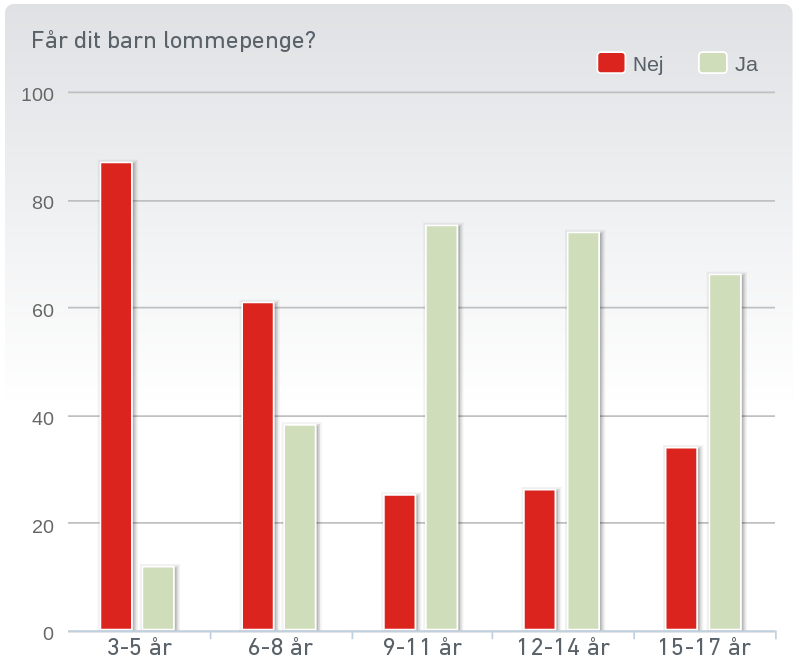
\includegraphics[width=0.7\textwidth]{Billeder/FaarBarnLommepenge.png}
\caption{Forældres svar på spørgsmålet '\textit{Får dit barn lommepenge?}'}
\label{FaarBarnLommepenge}
\end{figure}

\section{Lommepengemodeller}
\label{LommeModeller}
%Der findes mange forskellige typer børn og unge, 
%og derfor er det også meget forskelligt hvordan 
%disse unge lærer bedst. Dette betyder også at 
%der findes en række forskellige modeller for 
%hvordan lommepenge kan gives. I nogle modeller 
%skal børnene selv bidrage til de huslige pligter 
%for derved at gøre sig fortjent til 
%lommepengene, hvorimod andre modeller benytter 
%lommepenge som et tilskud, børnene og de unge 
%får et antal gange om året eller måneden. Hver 
%enkelt model har dog sine egne fordele og 
%ulemper, som vil blive fremhævet i dette afsnit. 
%De forskellige modeller er fundet hos danske 
%bank\cite{DanskeB2}\cite{DanskeB3}.

%\subsection{Model 1: Det rene tilskud}
%Ved denne model, vil børn og unge få det samme 
%beløb, et antal gange om måneden eller året. 
%Dette kan f.eks. være starten til hver måned 
%eller hver uge. Denne form for model kræver ikke 
%at børnene eller de unge har pligter.

%En af fordelene ved denne model, er at barnet 
%eller den unge får mulighed, for at koncentrere 
%sig om vigtigere ting på daværende tidspunkt, 
%som ikke vil være muligt at lære eller gøre 
%senere. Dette kan for eksempel være det sociale 
%liv eller lektier og skole, som nogen vil finde 
%vigtigere på et sådant tidspunkt.

%En ulempe ved denne model, er at manglen på 
%pligter kan give barnet det indtryk, at penge er 
%en selvfølge, som ikke behøves at skaffes gennem 
%arbejde. Dette kan gøre at barnet senere hen, 
%vil have svært ved at acceptere at skulle 
%arbejde for at få penge, og derved skabe et 
%såkaldt “luksusbarn” som forventer at blive 
%betalt uden at give noget igen, i form af 
%arbejde eller studieengagement.

%\subsection{Model 2: Lommepenge inkluderer 
%pligter}
%Denne model bygger oven på den forrige model ved 
%at inkludere faste pligter til børnene eller de 
%unge, som skal klares, for at lommepengene 
%bliver udbetalt.

%En fordel ved denne model, er i kontrast med 
%modsatte model, en forståelse for at man skal 
%arbejde for at få penge, og derved skaber et 
%bedre forhold til brugen af pengene i sig selv. 
%Et sådant forhold vil kunne hjælpe den unge 
%person, når han eller hun skal stå på egne ben 
%og styre sin egen økonomi, når denne person 
%flytter hjemmefra.

%En anden fordel ved denne model, er at det gør 
%børnene og de unge opmærksom på kravene for at 
%en husstand kan fungere og derved giver en 
%helhed i familien, som børnene bliver en del af. 
%Et sådant sammenhold vil ikke kun styrke 
%familien, men også give børnene en bedre fordel 
%ved fremtidige sociale forhold, hvor der også 
%stilles krav til dem.

%En ulempe ved denne model, er at børnene kan 
%vokse op med en forventning om udbetaling, for 
%hver enkelt gang de yder hjælp i 
%familiesammenhænge. Dette kan bevirke at børnene 
%enten kan begynde at kræve penge for alt hvad de 
%laver, eller at disse børn simpelthen ikke vil 
%lave noget udover, de pligter de blev påsat i 
%starten. Et sådant forhold til pligter og krav, 
%kan give en destruktiv adfærd, som ikke vil 
%gavne når barnet skal videre i sin dannelse.

\subsection{Model 3: Akkordmodellen}
Akkordmodellen bygger på forholdet mellem penge 
og arbejde, som der bliver benyttet i det 
virkelige liv. Penge vil blive udbetalt, for 
hver pligt i husstanden, der bliver løst. 
Beløbet som der udbetales kan være et fast beløb 
for alle pligter, eller det kan være et 
varierende beløb, som ændres efter varigheden af 
og sværhedsgraden pligten.

En af fordelene ved akkordmodellen, er dens 
mulighed for at give børnene og de unge, et 
indblik i den virkelige verdens økonomi, hvor 
der er sammenhæng mellem arbejdet og løn. Dette 
betyder således at de unge i fremtiden vil have 
nemmere ved at kunne se pointen i jobs, og 
derved skabe en tidlig lyst til at blive 
selvforsynende og dermed lære endnu mere om 
deres fremtidige økonomi.

En ulempe ved denne model, er at dennes krav til 
udbetaling for hver enkelt pligt, kan give 
barnet mistillid til familiens forhold, og at 
det vil kræve penge for at være en del af denne. 
Dette kan være en dårlig indstilling for 
fremtidige sociale udfordringer.

%\subsection{Model 4: Lommepenge et, pligter 
%noget andet}
%Denne model ser på lommepenge og huslige pligter 
%som to forskellige ting, som ikke skal have 
%nogen sammenhæng. Dette medfører dermed at 
%børnene, vil få lommepenge med et fast interval, 
%eller børnene har brug for det. Anden del af 
%denne model, betyder så også at det kræves af 
%børnene at et antal pligter bliver udført, men 
%mangel på denne udførsel, vil ikke påvirke 
%lommepengene.

%En fordel ved denne model, er at det giver 
%barnet et sammenhold med familien, og en 
%forståelse af hvordan en husstand har brug for 
%alles hjælp, for at kunne fungere, uden at der 
%skal gives lommepenge for de ting hver person 
%hjælper med. Dette vil også kunne hjælpe 
%fremover, ved sociale tidspunkter, hvor penge 
%ikke er et punkt, mens sammenholdet i en mulig 
%gruppe er.

%En ulempe som denne model giver, er det svage 
%billede af økonomien, barnet vil vokse op med. 
%Barnet vil se penge som en selvfølge og ikke se 
%sammenhængen mellem dets pligter og 
%lommepengene. Dette kan være med til at skabe et 
%dårligt forhold til penge i sig selv, og derved 
%skabe problemer for barnet eller den unge i sit 
%senere liv.

%Det ses at der ved hver model, både er fordele, 
%men også ulemper, der skal tages højde for, når 
%forældre vælger hvilken form for lommepenge, 
%deres børn skal have.



%\subsection{Vurdering af Lommepengemodeller}
%\label{ModelVurdering}
%Udfra det tidligere afsnit AFSNIT HENVISNING hvor vi så hvilke fordele og ulemper de forskellige lommepengemodeller giver, har vi opstillet en række vurderingskriterier, som de forskellige modeller skal bedømmes ud fra. Derefter kan de bedste modeller findes eller hvis muligt kan en eller flere modeller sammensættes og derved skabe en model, som vil opfylde kriterierne endnu bedre.

\uline{\textbf{Vurderingskriterier:}}

\\\textbf{1) Økonomisk forståelse}
Som det blev forklaret i afsnit AFSNIT HER er det vigtigt for de unge at få en forståelse af, hvordan økonomi foregår, og hvordan de senere i deres liv vil blive nødt til at arbejde for at kunne tjene penge. 
Disse kriterier medtager også forståelsen for at der er forskel på hvor meget arbejde der lægges i de forskellige opgaver, og dermed også forskel på udbetalingerne.
Dette kriterie bedømmer hvor god mulighed de unge får for at lære om den økonomiske del ved hjælp af den valgte lommepengemodel.

\\\textbf{2) Husstandsbidrag}
Sammenhold i familien og husstanden. 
Det er vigtigt for de unge at lære at fungere i en familie og mindre grupper. Dette betyder derfor også at de unge skal hjælpe til i deres husstand.
Dette kriterie bedømmer derved hvilken grad, den valgte lommepengemodel, giver de unge muligheder for at udvikle sine evner til at hjælpe i familien og det at være del af en gruppe.

\\\textbf{3) Tidskrav}
Hvor meget tid lommepengemodellen kræver af de unge.
Dette kriterie kigger på hvor krævende det, for de unge, vil være, at benytte den valgte lommepengemodel, og derved fjerne deres tid og koncentration fra andre emner der kunne være vigtigere. Hvis de unge ikke får tid til at udvikle sig socialt og skolemæssigt, vil de få det langt sværere i deres senere liv, end hvis de har en dårlig forståelse for økonomi.
Derfor er det vigtigt at bedømme hvor balanceret de forskellige lommepengemodeller er, så det ikke fjerner de unges fritid.

\\\textbf{4) Enkelthed}
Dette kriterium vurderer hvor svært det vil være for børne at benytte denne model, men også hvilken sværhedsgrad det vil give forældrene at opstille betingelserne og styre denne model.

\\\textbf{5) Digitaliserings relevans}
Dette kriterium vurderer i hvor høj grad det er relevant at fremstille en digitalisering af modellen. Dette vurderes ud fra hvor systematiseret modellen er. Ved systematisering forstås i hvor høj grad der er sammenhæng mellem det udbetalte beløb, og forventet udførelse%, samt et eller andet - ved ikke helt

Skemaet fungerer ved at der gives en bedømmelse fra 1-10 ved hver fordel. Derved vil hver lommepengemodel, have et antal point, som svarer til den samlede bedømmelse.

\\Model 1: Det rene tilskud
\\Model 2: Lommepenge inkluderer pligter
\\Model 3: Akkordmodellen
\\Model 4: Lommepenge et, pligter noget andet

\begin{center}
   \begin{tabular}{| l | l | l | l | l |} 
   \hline
   & Model 1 & Model 2 & Model 3 & Model 4 \\ \hline
   Økonomisk forståelse & 3 & 6 & 9 & 3 \\ \hline
   Husstandsbidrag & 1 & 6 & 6 & 8 \\ \hline
   Tidskrav (Højere er bedre) & 8 & 4 & 3 & 5 \\ \hline
   Enkelthed & 9 & 5 & 3 & 7 \\ \hline
   Digitaliserings relevans & 1 & 7 & 8 & 6 \\ \hline
   I alt & 22 & 24 & 29 & 29 \\ \hline
   \hline
   \end{tabular}
\end{center}


\section{Valuta}
\label{Valuta}
Dette afsnit kommer til at handle om hvilken slags valuta, som kan tages i brug af lommepengemodellerne. Der kommer til at blive argumenteret frem til eventuelle fordele og ulemper, ved de valuta former som er tilgængelige.

Systemet kan fungere mere i en retning der ligner et spil, hvor de penge, der er i omløb, ikke har nogen relevans til virkelig penge. Altså, der bliver gjort brug af en form for valuta inden for systemet, og børnene kan derefter handle med denne form for valuta, som de nu engang ønsker. På den anden side kan systemet også gøre brug af rigtige penge, i form af lommepenge, idet systemet allerede er forbundet med pligter og evt. andet i husholdningen.

\begin{figure}[htb]
\centering
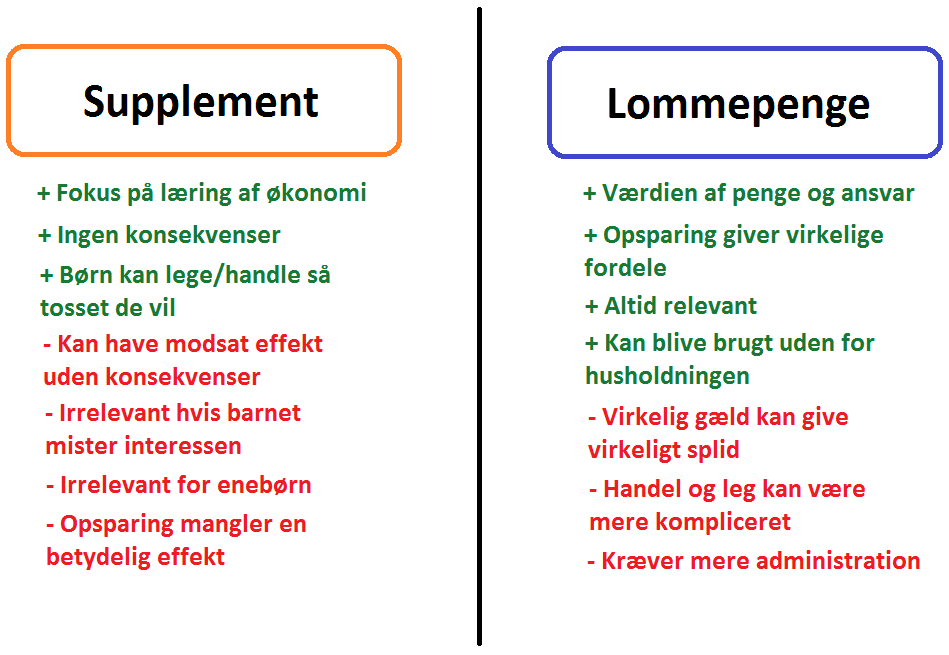
\includegraphics[width=0.8\textwidth]{Billeder/supplomme.png}
\caption{Fordele og Ulemper ved de to valuta former}
\label{SuppLomme}
\end{figure}

Systemet, som er baseret på sin egen valuta, kan have nogle fordele, når det kommer til at lære børn og unge omkring økonomi. Idet at systemet gør brug af sin egen fiktive valuta, som ikke har nogen sammenhæng med virkelige penge, så er der ingen større konsekvenser ved lån og minus på kontoen, som ellers ville være tilfældet med virkelige penge. Børnene kan derfor lege med systemet, og handle med hinanden, som de nu engang lyster. På den måde kan de også lære forskellige aspekter ved økonomi.

Det kan dog være, idet at der ikke er nogen konsekvenser ved systemet, at det kan have den modsatte effekt på barnet.  Systemet kan ende med at blive set mere som et middel i børnenes leg, i stedet for et værktøj til at lære dem om økonomi. På samme måde kan systemet ende med at blive irrelevant, hvis børnene bliver trætte af deres legetøj, eller mister interessen. Denne form for system, som fungerer som et supplement til lommepengene, vil have stor fokus på handlen der bliver gjort mellem børnene i dette system. Derfor vil systemet være stort set irrelevant for enebørn, som ikke har nogen søskende at handle med. Dette vil dog ikke være tilfældet hvis det er muligt at inkludere forældrene i systemet, og derfor også handlen. På samme måde mangler opsparing også en betydelig effekt, da det er en fiktiv valuta, og ville ellers bremse handlen og legen.
 
På den anden side har man et system, som er baseret omkring rigtige penge og er forbundet med de lommepenge, som børnene ellers ville have fået. Sådan et system, som sætter pengene sammen med opfyldelse af pligter, og giver rigtige penge der kan bruges uden for husholdningen, kan give en større fornemmelse af ansvar og den virkelige værdi af penge. Systemet kan ende med at give konstruktive lektioner angående økonomi, idet aspekter som renter og opsparing vil have en meget virkelig effekt. Denne form for system vil næsten altid være relevant, og vil sikkert kun blive mere relevant som barnet bliver ældre, idet selv børn har brug for penge.

Ulemperne ved dette system kan være, at det muligvis vil give splid i husholdningen, idet at gælden i systemet er baseret på virkelige penge. Handlen mellem søskende bliver også mere kompliceret, fordi der er virkelige penge på bordet, og giver heller ikke børnene den samme frihed for leg, som systemet lavet som et supplement har. Systemet baseret på penge kræver i sidste ende mere administration fra forældrenes side, sådan at børnene ikke ender med at sætte sig i gæld til skuldrene som 7-årige, udnytter sine muligvis yngre søskende, eller misbruger systemet.
 


\section{Projektafgrænsning}
Dette afsnit vil afgrænse projektets problemfelt, baseret på den foregående problemanalyse, for at finde en mere tydelige, specificeret og relevant målgruppe.

Der blev vist, at børn og unge har en utilstrækkelig forståelse for økonomi, selvom størstedelen modtager både undervisning og lommepenge. Ud fra afsnit \ref{Okonomi}  og \ref{LommeStat}  kan man umiddelbart se, at børn modtager undervisning i emner relevant til økonomi omkring slutningen af andet forløb i folkeskolen. Derudover kan man se ud fra statistikkerne, at indføring af lommepenge først rigtig slår ud omkring 9 til 11 års alderen, hvor antallet sprang fra 38 procent til 78 procent. Derudover er det omkring den samme alder, at børn begynder at lære om økonomi i skolen. Et supplement til læring af økonomi vil derfor være mest nyttigt omkring den samme tid. Derfor vil løsningen være rettet mod denne aldersgruppe.

I afsnit \ref{LommeModeller} blev der undersøgt forskellige lommepengemodeller, samt fordele og ulemper ved disse modeller. Derudover bliver der i det senere afsnit \ref{ModelVurdering} yderligere evalueret på disse lommepengemodeller, som viste at især ‘Akkordmodellen’ og ‘Lommepenge et, pligter noget andet’ står ud som de bedste af modellerne. Ud fra dette vil der blive afgrænset til at der skal implementere en eller muligvis flere modeller, baseret på de to førnævnte modeller, eller kombinationer mellem disse og eventuelle andre modeller. Helt præcis hvilke modeller der bliver taget i brug vil blive dækket yderligere i det kommende Design afsnit[[Ref når kapitel findes]], som skal prøve at finde frem til den bedste model, eller modeller, at implementere.

Til sidst er der afsnit \ref{Valuta}, som gør rede for fordelene og ulemperne, ved at basere en løsning på rigtige lommepenge, eller et fiktivt valutasystem. Begge sider af sagen har både mange positive og negative elementer til sig, så det er ikke helt klart hvad for en der vil fungere bedst i praksis, og give det bedst mulige svar på problemstillingen. Optimalt ville man prøve at implementerer begge muligheder, for at give flere muligheder til hvad brugeren kan med systemet. Dilemmaet her er at de to former er vidt forskellige, og skal derfor også implementeres og udvikles med vidt forskellige forhold i tankerne, som der ikke nødvendigvis er tid til. Derfor vil der umiddelbart blive afgrænset til et system baseret på rigtige lommepenge, som virker til at være bedre gearet til at lære om økonomi.

\section{Problemformulering}
Ud fra den forudgående problemanalyse er det blevet vist, at børn og unge har en utilstrækkelig forståelse for økonomiske elementer som renter, lån og opsparinger, samt en manglende forståelse for økonomisk ansvar. Alt dette er stadig tilfældet, selvom størstedelen af børn og unge modtager lommepenge fra deres forældre, samt undervisning i økonomiske elementer i deres skole, som begge gerne skulle have hjulpet dem til at have viden om økonomi. Derudover er der også blevet undersøgt og vurderet de forskellige versioner af lommepengemodeller, som forældre bruger til at udlevere og administrere lommepenge. På baggrund af dette problem, og den forudgående analyse af problemet, er der blevet udarbejdet følgende problemformulering:

\begin{itemize}

	\item Hvordan kan man lave et system a la et netbanksystem, på en datalogisk, som er baseret på lommepenge og pligter?
	\item Hvordan kan man lære børn og unge omkring økonomi, samt give en bedre forståelse for økonomi, ved hjælp af en datalogisk løsning?

\end{itemize}

Ud fra dette vil der blive arbejdet hen mod en prototype, baseret på objektorienteret programmering, der kan bruges som et værktøj til at understøtte børn og unges læring af økonomi.


%\section{Indlæringsalder}
%%\subsection{Hvor meget kan hver aldersgruppe lære?}
I dette afsnit vil der blive undersøgt hvornår børn lærer de færdigheder, som skal til for at kunne styre en privatøkonomi.

Undervisningsministeriet udgav i 2009 en serie hæfter med titlen Fælles Mål 2009, som beskriver hvad der forventes at eleverne lærer i de enkelte fag. En del af de Fælles Mål er, at beskrive trin for trin hvad der forventes af eleverne i de forskellige forløb i folkeskolen. Folkeskolen er inddelt i 4 forløb;
\begin{itemize}
\item 1.-3. klasse er forløb 1.
\item 4.-6. klasse er forløb 2.
\item 7.-9. klasse er forløb 3.
\item 10. klasse er forløb 4.
\end{itemize}

\emph{Efter 6. klasse}
%linebreak here
I faget matematik er det forventet at elever efter 6. klasse skal kunne regne med procenter, 
nærmere bestemt skal de: “kende procentbegrebet og bruge enkel procentregning”[[CITAT]]\cite{FallesMalMatematik}
Dette er naturligvis vigtigt da det er en forudsætning for at kunne regne med og forstå renter.

%en blank linje her...?
\emph{Efter 9. klasse}
%linebreak here
I matematik er det forventet at elever efter 9. klasse skal kunne regne med lønopgørelser, skatteberegninger og rentebegrebet.\cite{FallesMalMatematik} Sammen med rentebegrebet hører blandt andet også opsparing, låntagning og kreditkøb.
I samfundsfag, som i folkeskolen starter i 7- klasse, skal elever efter endt forløb kunne blandt andet: “Redegøre for det økonomiske kredsløb og markedsmekanismer”[[CITAT]]\cite{FallesMalSamfundsfag}
Dette indebærer blandt andet at eleverne skal kunne forstå begreber som lån, lønseddel, opsparing og husholdning.

[[En eller anden form for konklusion??;
Vi kan se at unge skal, i skolen, lære om procenter omkring år 11-12, og derfor... bla bla ]]


\newpage
\thispagestyle{empty}
\mbox{}

% Kilder
\bibliographystyle{plain}
\bibliography{Referencer}

\end{document}
